% EPL master thesis covers template
\documentclass{eplmastersthesis}
\usepackage{float}
\usepackage{xcolor}

% Please fill in the following boxes
% Title of the thesis
\title{Integrated mini-cloud of RaspberryPIs for distributed systems training}

% Subtitle - remove this line if not applicable
\subtitle{The Splay Project}

% Name of the student author(s)
\author{Rémy \textsc{Voet}}
\secondauthor{Samuel \textsc{Monroe}}		% remove if not applicable
%\thirdauthor{Firstname \textsc{Lastname}}			% remove if not applicable

% Official title of the master degree (copy/paste from list below)
% Master [120] in Biomedical Engineering
% Master [120] in Chemical and Materials Engineering
% Master [120] in Civil Engineering
% Master [120] in Computer Science
% Master [120] in Computer Science and Engineering
% Master [120] in Cybersecurity
% Master [120] in Data Sciences Engineering
% Master [120] in Data Science: Information technology
% Master [120] in Electrical Engineering
% Master [120] in Electro-mechanical Engineering
% Master [120] in Mathematical Engineering
% Master [120] in Mechanical Engineering
% Master [120] in Physical Engineering
% Master [60] in Computer Science
% Specialised master in nanotechnologies
% Specialised master in nuclear engineering
\degreetitle{Master [120] in Computer Science}

% Name of the supervisor(s)
\supervisor{Étienne \textsc{Rivière}}
%\secondsupervisor{Firstname \textsc{Lastname}}		% remove if not applicable
%\thirdsupervisor{Firstname \textsc{Lastname}}		% remove if not applicable

% Name of the reader(s)
\readerone{Firstname \textsc{Lastname}}
\readertwo{Firstname \textsc{Lastname}}			% remove if not applicable
\readerthree{Firstname \textsc{Lastname}}			% remove if not applicable
%\readerfour{Firstname \textsc{Lastname}}			% remove if not applicable
%\readerfive{Firstname \textsc{Lastname}}			% remove if not applicable

% Academic year (update if necessary)
\years{2018--2019}

% Document
\begin{document}
  % Front cover page
  \maketitle

  \chapter*{Abstract}

  \chapter*{Acknowledgements}

  \tableofcontents

  \chapter{Introduction}

    \section{Context and Motivations}

      {\color{red} Rewrite and complete this, placeholder right now}\\

      The process of learning distributed systems and algorithms is usually
      undermined by the difficulty of being able for one to test and apply
      what he learns.\\
      Indeed, in order to run a distributed algorithm and observe the result, a
      collection of machines running the algorithm is needed. Besides that,
      one would like to be able to change the conditions in which the algorithm
      is run, for example by provoking faulty nodes, or inducing network
      perturbations among the system, as distributed algorithms are designed to
      adapt to these conditions. These needs make it really cumbersome
      for students to setup a testing environment emulating realistic
      conditions for learning purposes.

    \section{About the Splay Project}

      % Discussion about what was available when we started the rework of the Splay project.
      The SPLAY project has initiated to solve the difficulty to test and develop distributed algorithm in a large scale. SPLAY is not a recent project (begin around 2006), and lot of features have been added during some years. The first version of SPLAY  was designed to "covers all aspects of the development and evaluation chain" of distributed application \cite{SPLAY}. \\

      After some years, a module has been constructed be to manage network topology, SplayNet \cite{SplayNet}. This middleware implements a easy way to set the topology network between the endpoints (machines) and restrict the usage of the network depending of that.

      \subsection{Legacy Splay Project}

        When we begin our work on Splay, the repository of the project \cite{SplayGit} was not consistent. Indeed, the master branch is unstable, ...

      \subsection{A first update}

        Nous avons eu la chance d'obtenir auprès de l'UCL un travail étudiant
        en lien direct avec ce mémoire. Il s'agissait, à l'issue de dix jours
        de travail, de mettre à jour la version des technologies utilisées par
        Splay et par la même occasion acquérir une connaissance plus complète
        du fonctionnement du projet.\\

        Lors du début du travail, les derniers updates sur le projet dataient
        de 2016, et un certain nombres de features et améliorations avaient
        été développés jusque là. Cependant le projet n'était pas dans un
        état stable et donc Raziel Carvajal Gomez (notre superviseur pour ce
        travail contributeur de Splay) a préféré nous faire faire un fork
        du projet sur un commit remontant en Septembre 2011.\\
        Nous avions donc le bénéfice de repartir sur des bases saines et
        un projet fonctionnel, mais avec une grande perte en ce qui concerne
        le travail qui avait été accompli sur les cinq années qui séparent
        2011 de 2016.\\
        C'est là que nous avons relevé le premier problème
        et élément que nous voulions absolument changer et intégrer dans notre
        reprise de Splay: le projet avait été transferé depuis son ancien
        système de versionning sur Git et uploadé sur Github en Juin 2011 mais
        n'avait pas profité du système de tag de versions offert par Git pour
        référencer dans l'histoire du projet des releases fonctionnelles
        et stables, c'est donc quelque chose que nous mettrions en oeuvre
        par la suite.\\

        Partant de là, nous avons pu nous familiariser progressivement avec
        le fonctionnement du projet et son architecture software, appréhender
        les différents services qui le composaient et comprendre leurs
        interactions. Une fois cette connaissance acquise, nous avons pu
        commencer à upgrader les différentes versions des technologies
        utilisées en commencant par le Ruby et le Lua, les deux plus importantes
        et plus présentes technologies du projet.\\
        Avec des versions datant de 2011 maximum, et étant donné que nous voulions
        transiter sur les versions les plus récentes disponibles, nous savions
        pertinamment qu'au moment où nous changerions les versions, le projet
        deviendrait totalement instables et que de nombreux appels de méthodes
        ou fonctions dépréciées seraient à changer avant de récupérer un état
        stable. Mais là aussi nous avons relevé un second problème et élément
        primordial à intégrer pour les futures améliorations, le projet
        manquait cruellement de tests, à quelque niveau que ce soit.\\

        La conséquence de ceci était que nous devions réparer pas à pas le
        projet suite au changement des versions des langages et frameworks en
        devant nous baser sur notre compréhension globale du projet acquise
        précédemment et sur des resultats finaux attendus lors de l'exécution
        de divers scénarios utilisant le projet. Il nous était impossible d'être
        certains que nos changements n'affectaient pas le fonctionnement interne
        du projet de manière négative mais imperceptible, conséquences qui
        étaient en fait inévitables mais que nous ne découvririons que par
        la suite lors de l'implémentation de nouvelles features.\\
        Il était dès lors évident pour nous que nous mettrions en place des
        séries de tests à plusieurs niveaux lors des prochaines phases du
        projet, afin de rendre celui-ci bien plus maintenable que dans l'état
        où nous l'avons repris et de pouvoir garantir de futures améliorations
        plus aisées.\\

        Nous sommes donc parvenus à progressivement remettre en état (partiellement avec la feature principal) de
        fonctionnement tous les éléments composant Splay avec les nouvelles
        versions, en mettant également à jour les librairies utilisées par
        les différents langages. Les changements principaux en termes de
        version de technologies sont les suivants :

        \begin{itemize}
          \item \textbf{Ruby}: 1.8.6 $\rightarrow$ 2.5.3
          \item \textbf{Lua}: 5.1 $\rightarrow$ 5.3
          \item \textbf{Rails}: 2.1.0 $\rightarrow$ 5.2.0
          % Eux, ça s'était après :
          % \item \textbf{MySQL}: 5.5 $\rightarrow$ 5.7
        \end{itemize}

        Nous avions à l'issue de ces dix jours de travail une base saine et
        mise à jour prête à être utilisée pour le travail concret de notre
        mémoire.\\

        En plus de ceci, une autre partie du travail a consisté, une fois les
        updates réalisés, à mettre à jour la documentation du projet et y
        décrire le fonctionnement des différents services ainsi que de prendre
        du temps afin de réfléchir à des améliorations au niveau de
        l'architecture du système et de son fonctionnement et avons émis
        les réflexions suivantes :

        \begin{itemize}
          \item L'organisation du code n'était vraiment pas idéale et devrait
          être changée. Le code des six différents services se trouvait dans
          un seul même repository, ce qui rendait compliqués la navigation dans
          l'arborescence du projet pendant le développement, le suivi des
          commits et donc de l'évolution de ces différents services.
          \item Le fait d'utiliser une database comme point de communication
          entre le côté user et le \textbf{Controller} n'était peut-être
          pas aujourd'hui la meilleure manière de procéder.
          \item L'utilisation de Ruby comme langage pour le \textbf{Controller}
          et de LUA pour les \textbf{Daemons} n'était peut-être plus
          aujourd'hui un choix pertinant et des alternatives possibles
          pour des applications multi-processus et concurrentielles telles
          que Elixir demandaient analyse. Un différent choix de technologie
          aurait aussi pu par la même occasion solutionner notre interrogation
          précédente sur la base de données.
        \end{itemize}

        Ces réflexions ont été ensuite discutée avec Etienne Rivière, afin de
        dresser ensuite le ligne directrice et les objectifs concrets à atteindre
        pour la suite du projet et entammer la version 2 de Splay.

  \chapter{Splay Version 2}

    % All about what we wanted to do exactly.
    Then, our goal for the new version of Splay, was first, stabilize and modernize the legacy project. Indeed, some parts was not updated or partially documented. All details is available in the next section.\\

    In a second step, we wanted to add our own features focus on the usage of the final user (student, professor or searcher). These features were a modern web application with Lua editor integrated, a graphical topology creator inside the web app and a way to inject some fault injection in the user code. We will details all of then in this chapter.

    \section{Objectives}

      % Adding features of splayNet with
      Our Objectives can be easily cup in two parts, first the maintainability of the project and the new features added (next section). The section about our first update during a student job, explains the upgrade of language version but this upgrade was not covered all features of the legacy project (example: SplayNet). Then our first job was to\textbf{ complete the missing features} done after  September 2011. \\

      % Raspberry
      The first idea of our master thesis was able to run Splay on a \textbf{cluster of Raspberry Pi}. The configuration of this cluster won't be trivial : one Raspberry need to be the master and able to control the rest of the cluster. Then the master need to run the controller and the web application and the other need to be handle to manage several Splay daemon (use as a machine for the distributed algorithms). \\

      % Clean code source - repo
      Secondly, Splay is not a small project, and several technologies (services) orchestrated between then. For this reason, the source code architecture is very important for the project maintainability. In the legacy project all code was on a single git repository host on Github, but this one is a "mess". The documentation is not in the right place, the logic of the directory structure is too complex, ... Then we wanted to do a better \textbf{management of the source code} and documentation readable by someone finding our repository. \\

      % Easy installation : On click install : docker (independent of OS), installation script,
      During our first work on Splay, we noticed that the installation and the usage was not quite easy to handle. Some services were dockerize and a docker-compose file was implemented which facilitate the installation. But these docker images were not perfectly build : healthcheck missing, old base image in some cases or big distribution base image (slow and take place). Also there wasn't a proper \textbf{one-click install} script for making quick test. Then, one of our goal was to get clean, small and with updated libraries docker images. These images need to be fully integrated between then through the docker-compose. A automate install script and running script, will be appreciate and useful as a example for the user.\\

      % Bug track - Testing - Solve issues of the old project
      Our first issues encounter with Splay, was the lack of \textbf{automatic tests} in all part of the project and because of this, there were a lot of silent bugs scattered in all the project. Accordingly, we wanted to upgrade the robustness of the project, it is means create specific test for critical parts and the main features of Splay. Two type of test can be created, local testing and integration testing. The first type allows to test a specific critical part or feature of one service (independently of others). The second kind is testing the global project by simulate a real user and getting real result from Splay (able to test the chain of service). The goal of these test is a better bug track and create maintainable project for future development.\\

      % Merge Web app and Cli server + new web app
      During our student job, we observed some code repetition and service repetition (cli server and the old web application). Then,we wanted to \textbf{avoid the repetition of job} (and code by extension) by change these services or merge it. Again, the purpose was the maintainability and refactor some old code. Moreover, we wanted to modernize the web application of the legacy project and add some features on it (next section)


    \section{New features of Splay}

     To present our own new features of Splay, we will explain by some user scenarios and after explain in details the three features.

      \subsection{Scenarios}

        \textbf{First Scenario : } as a student, I want to put in practice my course on distributed application. The university provides a existing installation of Splay in the local network. The student just need to connect on the web server with its browser. The student, after registering, will able to create its own code with a complete Lua editor on the web page. Also a powerful and documented library facilitates the creation of distributed algorithm. When the code is finished, the student launch the job, the code will be automatically dispatch on several machines (depending of number of available daemon and the number choose by the student), and getting the log of each of then in the web page during/after the completion of the algorithm. Also, if it is too long the student can choose to kill the job. The student, through a simple web interface, can put in practice its course and see the result quickly via logs.\\

    	\textbf{Second scenario : } a professor wants to test a new approach to solve the problem of leader election between multiples nodes. A cluster of Raspberry is set up with Splay to make the experiment. The new approach is described in a paper with some pseudo-code and some difficult cases when the network topology is quite exotic. Then the professor need to rewrite the pseudo code in a actual one and create a simulation or truely the different exotic network topology to point the strength of this new approach. Unfortunately, He is very busy, and it time is very precious. It is case Splay can be the solution, it manages network topology transparently and give a topology creator in a web page. Also the library of Splay in the Lua side allow to quickly reproduce the pseudo-code.

        % \textbf{Third scenario : } A employee from a big cloud company want to test the robustness of their new Top Secret distributed algorithm. TODO

        % as a employee from a cloud company who want test the robusness of their new Top Secret algorithm.

\subsection{Details of features}

\subsubsection{Complete Lua editor on the website}

Splay in version 1, had a web application, with some basics features : user connection, list of job, creation of job and a way to retrieve logs. This web application as explained before was very trivial with almost no CSS and poor in term of content. Then, we wanted to refactor completely and modernize the old web application. And, also in this purpose, the user could use a integrated Lua editor directly on the website. This editor should be standalone, with coloration for Lua language, error parsing and maybe some small auto-completion. This one need to be integrated into the form of the job creation.

\subsubsection{Topology creator/visualisation}

Also, the legacy project manages network topology. Indeed a user can defined its own network topology with different settings for each edge : the latency, the bandwidth and error dropping packet. Also it is possible to make more complex network by adding router between nodes and Splay will approximate the true parameters for each source-destination (Splay will not simulate the internal node of the network, for performance reason and simplicity). \\

The network settings is done on the legacy project by a XML file with a specific format (ModelNet \cite{ModelNet}). This format is not user friendly and hard to read, also the documentation is poor. For these reason, we decided to add a visualization and creation tool of the network graph. Then, it will be possible to create easily a visual topology with all type of setting and it will be transform automatically in the correct format of XML. But, the opposite will be possible, it means from a XML, see the topology into a graph representation.

\subsubsection{Fault Injection}

The creation of distributed algorithm is a difficult task, and moreover, it is hard to make real code who is reliable. Robustness and correctness of a distributed solution is the key point to test for a designed solution, and manually injection of fault is painful and can take some time. \\

With the legacy project and the dockerization, it was possible to crash a single daemon during the execution of a job. But the main problem of this solution, we can't control where the crash is done (in the execution tree). We wanted to improve this precision by adding a feature where the user is able to choose when a daemon (or several) crash during the execution of code. It need to convert the two main different, the hard crash (the nodes is destroyed) or a recovery crash (nodes crash but it is relaunch after some time). \\

To resume, the fault injection will allow (user) to choose when (in the execution tree) and where (one or several nodes) the crash is done in the daemon, specified the type of crash and act depending. This possibility for the user need to be user friendly and quick to make.

% This for reason - 2 types of crash possible - can touch one or more than one in the same time - crash in middle 2 instruction.

  \chapter{Architecture}

    \section{Software Architecture}

      It is important here to discuss about the software architecture of the
      Splay Project as it has impacts on the way we achieved this work

      \subsection{Legacy Architecture}

        The old Splay architecture was composed of :

        \begin{itemize}
          \item The \textbf{Controller} : The core part of Splay, waits for jobs
          and dispatch them to the daemons.
          \item \textbf{Daemons} : Workers registering to the controller and waiting
          for jobs to achieve.
          \item A \textbf{MySQL DB} : The communication piece of Splay, allowing
          communication between the user and the system.
          \item A \textbf{CLI Server, CLI Client, SplayWeb} : Pair of CLI tools
          and a web application made in Rails to let user interact with
          Splay through communication with the MySQL Database.
        \end{itemize}

        % Figure of the old architecture, TODO : remake with technologies used
        \begin{figure}[H]
          \centering
          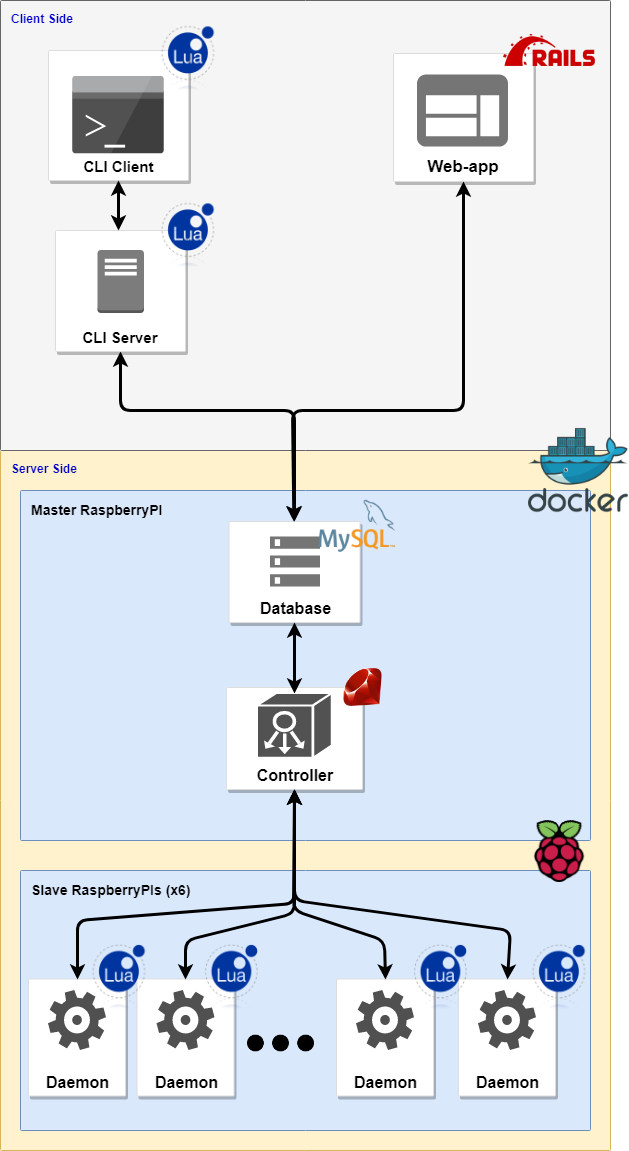
\includegraphics[scale=0.6]{figures/prev_arch.png}
          \caption{\label{prev_arch} Previous Splay Architecture}
        \end{figure}

        Que cela soit à travers l'utilisation du CLI ou de l'application SplayWeb,
        un utilisateur pouvait intéragir avec Splay et y envoyer ses jobs, récupérer
        des informations telles que les logs ou l'état des Splayds.\\

        Le fait que la base de données soit l'élément central de communication entre
        le contrôleur et les applications utilisteurs était un choix de design
        que nous avons choisi de respecter. En effet, le \textbf{Controller} est
        l'élément central du projet Splay, vouloir apporter un changement dans ce choix
        de design et opter pour un remplacement de la façon de communication aurait
        impliqué plus que certainement une réécriture quasi totale du contrôleur.\\

        Cela dit, nous n'étions pas satisfaits par les possibilités d'interactions
        offertes à l'utilisateur. En effet, l'application Ruby on Rails était assez
        vieille, et la paire client/server du command-line-interface possédait une
        codebase difficile à maintenir et trop imposante pour les features qu'elle
        devait proposer.\\

        Nous avons donc choisi d'opérer des changements majeurs sur cette partie
        du projet Splay, afin d'en plus d'opérer les changements et ajouts de features,
        proposer une bonne expérience utilisateur.

      \subsection{Renewed Architecture}

        Le principal problème du côté de l'architecture des services utilisateurs
        était la duplication de code, ou du moins une duplications des solutions
        apportées pour un seul et même problème. L'application web Rails et le
        serveur CLI avaient en commun la manipulation de la base de données pour
        transmettre et récupérer les informations au \textbf{Controller} pour
        le compte de l'utilisateur.\\

        La première décision à prendre pour pallier à ce problème était de
        fusionner ces deux services en un seul et de l'appeler selon sa responsabilité
        au sein du système, le \textbf{backend} d'un point de vue client.\\
        Ce backend aurait pour ambition de proposer une API sécurisée via
        JsonWebToken et permettant ainsi la construction de services autour de
        ce backend, en l'occurence une application web et un client en ligne
        de commande.\\

        L'application web utiliserait donc une technologie JavaScript récente
        permettant des interactions dynamiques avec l'utilisateur, et le CLI
        une technologie simple et adaptée, les deux consommant l'API fournie
        par le backend. Ce backend resterait quant à lui dans l'écosystème Ruby,
        pour garder une consistance avec le projet tel qu'il était.\\

        On obtiendrait donc l'architecture retravaillée suivante :

        \begin{itemize}
          \item The \textbf{Controller} : The core part of Splay, waits for jobs
          and dispatch them to the daemons.
          \item \textbf{Daemons} : Workers registering to the controller and waiting
          for jobs to achieve.
          \item A \textbf{MySQL DB} : The communication piece of Splay, allowing
          communication between the user and the system.
          \item \textbf{Backend} : The backend of the client side Splay app
          \item A \textbf{Web-app} : The single-page application
          \item A \textbf{CLI} : The command-line interface
        \end{itemize}

        \begin{figure}[H]
          \centering
          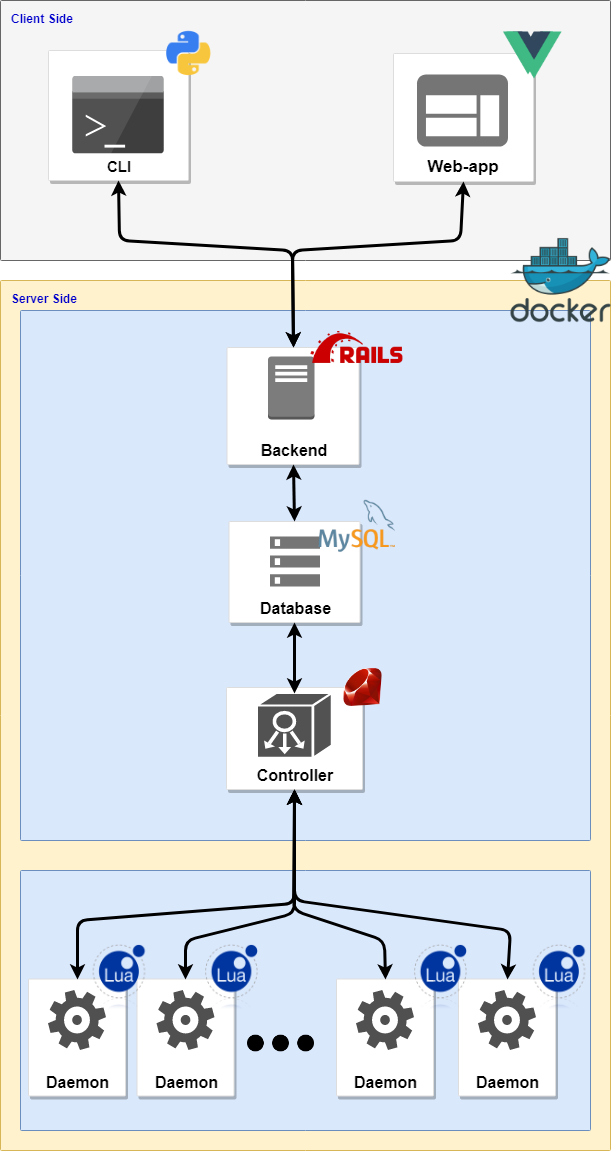
\includegraphics[scale=0.125]{figures/new_arch.png}
          \caption{\label{new_arch} New Splay Architecture}
        \end{figure}

    \section{Hardware Architecture}

      About the Rasp cluster.

  \chapter{Development Methodology}

    Avant de parler des détails d'implémentation, il est utile de décrire la
    façon dont nous nous sommes organisés afin de développer l'application, le
    fait d'être deux à faire ce travail nécessitait forcément une façon de
    s'organiser un peu plus sérieuse qu'un développement seul.\\

    Grâce à des cours suivis pendant notre cursus au sujet de méthodologies
    AGILES, et ayant tous deux eu l'occasion d'acquérir de l'expérience de manière
    professionnelle au travers de stages et de part-times jobs, nous avons
    voulu mettre à l'oeuvre ces connaissances et bonnes pratiques acquises dans
    le domaine de la gestion de projet.

      \section{Kanban}

        Le premier outil que nous avons mis en place, et ce dès notre période
        d'update de Splay dont nous avons parlé plus tôt, a été un Kanban en
        utilisant le site en ligne Trello. Le kanban nous a permis de : \\

        \begin{itemize}
          \item Avoir une vue claire et précise sur les tâches à accomplir restantes
          dans le backlog, ainsi que de l'état de développement des autres tâches.
          \item Nous pousser à traduire les features à réaliser en cartes
          suffisamment détaillées et explicites, pouvant aboutir à des clarifications
          ou refontes de certaines features avant le début de leur développement.
          \item Avoir un moyen de tracking de l'avancement du projet et fournir aux
           personnes impliquées dans le projet Splay un moyen simple et efficace
           de se tenir informer sur l'état de Splay.
          \item Se concentrer sur des tâches spécifiques et travailler de manière
          itérative et efficace.
        \end{itemize}

      \section{Quality Assurance}

        Ceci sera explicité plus en détail dans un chapitre suivant, mais nous
        avons voulu nous assurer de maintenir un certain degré de qualité dans
        notre travail sur Splay et plus spécifiquement au niveau du code, afin
        aussi d'assurer la maintenabilité du projet. Nous nous sommes donc
        fixés ce but à travers la mise en place des éléments suivants : \\

        \begin{itemize}
          \item \textbf{Testing suites} : Ensembles de tests unitaires et
          d'intégration, intra-service et inter-services.
          \item \textbf{Linter} : Analyse statique du code afin de satisfaire à
          des exigeances de style de code et de bonnes pratiques.
          \item \textbf{Coverage Analyzers} : Analyse du pourcentage de couverture
          du code par les suites de tests.
        \end{itemize}

      \section{Github and Gitflow}

        Le projet et les divers services qui le composent sont versionnés
        en utilisant le système de versionning \textit{Git} et hostés
        sur le service en ligne \textit{Github}.
        Nous avons donc organisés notre travail sur le modèle du Gitflow.
        Chaque feature ou tâche que nous avions créée sur le kanban était
        destinée à recevoir sa propre branche, partant de la branche principale.
        Une fois la feature terminée et testée, une pull request était créée
        demandant la fusion de la branche de feature sur la branche principale.
        Le bénéfice premier étant évidemment de garder la branche principale
        dans un état fonctionnel avec des features implémentées terminées et
        saines.\\

        Le deuxième atout de cette méthode de travail au sein de notre groupe
        était de pouvoir, encore dans un but d'assurer la qualité, aisément
        organiser du reviewing de code entre nous. Chaque fois qu'un de nous
        finissait une tâche et effectuait une pull request, l'autre était
        assigné en tant que reviewer et chargé d'accepter la pull request
        et d'effectuer le merge, ou détecter des erreurs à l'issue de cette
        review et de demander les changements adéquats au premier.\\
        Outre le bénéfice premier de la review dans la réduction du nombre
        de bugs ou d'erreurs, cela permettait aussi à chacun d'entre nous
        de rester au courant de tous les changements au sein des différents
        services, puisque nous ne pouvions pas décemment travailler ensemble
        sur chaque service individuellement étant donné leur nombre et les
        features inter-dépendantes à développer.


  \chapter{Implementation}

    \begin{itemize}
      \item Détails sur les choix d'implémentation
      \item Story-telling sur le développement en lui-même
      \item Détails de l'implementation, comment Splay fonctionne aujourd'hui
    \end{itemize}

    \section{Technology choices}

      \subsection{VueJS - Web App}

        Puisque nous avions décidé que l'application web utilisateur se
        destinait à être uniquement une application front-end tirant
        parti d'un backend centralisé fournissant une JsonAPI complète, nous
        voulions utiliser un framework web front-end qui satisferait aux
        conditions suivantes : \\

        \begin{itemize}
          \item Léger
          \item Facilité de développement et de maintenance
          \item Accès à de nombreuses librairies tierces
        \end{itemize}

        Pour une application front-end, l'écosystème JavaScript était
        évidemment évident, et nos avis se sont de fait tournés vers
        les options ReactJS, Angular et VueJS, tous étant des framework
        populaires et reconnus pour leurs qualités.\\
        Nous avons vite évincé Angular car nous préférions l'orientation
        composant des deux autres frameworks, moins lourds et évitant
        ainsi de devoir composer avec une couche style MVC des apps Angular.
        Bien qu'ayant eu tous deux une expérience préalable avec le React
        durant nos cours de Cloud Computing au sein de l'UCL, nous avons
        décidé d'opter pour Vue au lieu de React.\\

        Le premier gros avantage de Vue étant sa légereté, nous avons
        aussi pris en compte le fait que la technologie gagnait en popularité
        depuis un certain nombres d'années pour être aujourd'hui un poids fort
        dans les technologies web. De plus, ayant pris le temps de d'essayer
        le développement d'une petite application test pour nous décider, nous
        avons été grandement satisfaits par la simplicité de développement que
        le framework Vue offre aux développeurs et nous permet d'être
        totalement confiant dans le fait qu'opter pour cette technologie
        permettra à tout contributeur de Splay de très vite pouvoir s'y
        retrouver et participer au développement.\\
        En effet, l'application se découpe sous forme de composants individuels
        possédant chacun leur template HTML, leur styles CSS et le script
        JavaScript associé. Aucun autre langage exotique n'est requis.\\
        Le fait que le framework se trouve dans l'ecosystème JavaScript et
        associé à NPM permet aussi de tirer profit de nombreuses librairies
        existantes, que ce soit au niveau du testing, de librairies de
        visualisation de données, etc...\\

        Pour toutes ces raisons, Vue s'est révélé être le choix ideal pour
        l'application web, et nous permettant en plus d'associer le bénéfice
        d'un développement agréable sur de nouvelles technologies en plus
        d'apporter une solution efficace aux requirements du service.

      \subsection{Python - CLI}

        L'ancienne paire de service destinés au CLI était écrite en LUA d'une
        part pour le côté client, et le serveur CLI en Ruby. Etant donné que
        la logique du serveur allait être déplacée dans le \textbf{Backend},
        et que nous voulions garder une application en ligne de commande
        pour des tests rapides de toute l'infrastructure, nous avons eu besoin
        de réévaluer la pertinence de l'utilisation du LUA pour cette application.\\

        Il est plus que probable que le LUA ait été utilisé à l'époque pour
        des raisons de cohérence, et pour éviter de disperser Splay autour
        de beaucoup trop de technologies différentes (bien que Ruby aurait
        aussi pu être utilisé). Toujours est-il que ce choix n'était aujourd'hui
        plus le plus pertinant pour une application de ce type, en effet notre
        petite application CLI client devait être : \\

        \begin{itemize}
          \item Simple
          \item Très concise
          \item Ecrite dans un langage facile d'utilisation
          \item Disposer dans l'idéal de librairies permettant la création
          de ce genre d'application
        \end{itemize}

        Hors nous avions hérité d'une application décomposée sur de multiples
        fichiers LUA, chacun représentant une commande. On avait donc
        énormément de duplication de code au niveau de la façon de parser
        les arguments et aussi dans la manière de contacter le serveur
        via une librairie HTTP de LUA.\\
        Ruby était évidemment une option valable si nous voulions restreindre
        le nombre de technologies différentes utilisées, mais Python se prêtait
        beaucoup plus à l'écriture d'un script simple tel que notre CLI, avec
        à disposition des librairies éprouvées pour ce qui est des requêtes
        HTTP et de la gestion de paramètres utilisateurs.

      \subsection{Ruby on Rails - Backend}

        Le controller et l'ancienne paire de services destinés au CLI ayant été
        développé en Ruby, et l'ancienne application web en Ruby on Rails, il
        nous semblait évident de rester dans l'écosystème Ruby pour créer
        le service qui deviendrait ce que nous avons appelé \textbf{Backend}.
        La technologie que nous voulions utiliser pour développer le backend
        devait proposer une solution efficace aux problèmes suivants : \\

        \begin{itemize}
          \item Permettre un interfacage simple avec la base de données MySQL
          pour assurer la communication avec le controlleur, et ainsi pouvoir
          soumettre de nouveaux jobs, récupérer les infos sur les Daemons, etc...
          \item Permettre de développer et exposer une JSON API permettant
          aux services front-end (application web et CLI) de l'exploiter
          pour interagir avec le système Splay.
          \item Offrir un large choix au niveau de librairies de testing,
          de serialization des données en JSON, et autres librairies permettant
          de répondre aux problèmes susmentionnés.
        \end{itemize}

        Ayant déjà tous deux une expérience assez conséquente en Ruby on Rails,
        et pour les raisons de consistance d'écosystème exposée plus haut, nous
        nous sommes immédiatement accordés pour utiliser cette technologie.
        Le fait de rester dans le même ecosystème de langage nous assurait
        aussi que les futurs contributeurs de l'application n'auraient pas
        à devoir jongler avec plusieurs technologies et faciliterait donc
        l'évolution future de Splay.\\
        Il est aussi à noter que comme nous l'avons explicité dans la partie
        concernant le renouvellement de l'architecture de Splay, la précédente
        web application et le serveur CLI avaient un rôle similaire bien que
        spécialisé pour différentes applications. Cependant la logique commune
        deux deux services en Ruby était déjà présente, et il s'agissait donc
        en partie de l'isoler et de l'améliorer.\\

        Rails permet en effet très simplement de développer, outre des
        applications web traditionnelles MVC, des applications destinées uniquement
        à être des API faisant fi de toute la complexité nécessaire à la
        présentation des vues pour l'utilisateur et donc légères et concises
        en terme de codebase.\\
        L'ORM ActiveRecord associé aux applications Rails était également un
        atout majeur pour cette technologie, nous permettant de gérer
        simplement et efficacement les jobs et daemons du système.\\
        Enfin, des librairies telles que RSpec pour le testing (point sur
        lequel nous reviendrons plus tard dans un chapitre dédié), Rubocop pour
        le linter, ou encore la libraire fast\_jsonapi de Netflix pour la
        serialization des données faisait vraiment de Rails la bonne technologie
        à choisir pour le Backend.

    \section{Development}

      This section details all step of our develop begin by the cleaning and refactoring of the
      legacy project and finishing by adding our own features. Note that the sections isn't a timeline
      of the final work, we didn't wait to finish one part to begin the next one (sort by work beginning),
      and some goal has been improved during the completion of the next one (or last one).

      \subsection{Github Repository}

        Our first goal was to get a clean github repository. We found the layout of the old project messy
        and for a possible user, it is difficult to understand how to use Splay and moreover how to install it. \\

        Our first solution idea was to fork the old project, arrange directories/files and add
        some documentation. After we did this, we felt that it wasn't good enougth. The project is big,
        and there are multiple services dependent but not sharing anycode. Then we decided to create multiple
        repository for the project : one for the main project and one for each part. The main project,
        called splay, contains the others with the submodule \cite{GitSubmodules} feature of git.
        These children repositories are 5, and represent the new architecture wanted :
        cli (command line interface), daemon (also called in the project splayd), backend
        (the merge of the cli\_server and the backend of the old web server), controller
        and one for the new front-end web application. \\

        Besides, each repository is self-sufficient, contains a Dockerfile allowing to create a
        insolate environment and some readme file is scattered in repositories.
        Also, each master branch of repository expect the main one, is linked with
        Dockerhub, after a push on the master branch, Dockerhub will automatical create a new images from
        the source and updated the lasted image \cite{DockerHubGithub}.

      \subsection{Centralization of Splay's Backend}

        How we moved the old rails app and cli server to a single backend
        to serve any app wanting to connect with Splay.

      \subsection{A new front-end application}

        As backend was available, development of a VueJS SPA.

      \subsection{Rework of the CLI to use new Backend}

        All the Command line interface has been redone in Python more clearly and concise.

      \subsection{Topology creation through Javascript Interface}

      \subsection{Fault injection}

    \section{Implementation Details}

      A precise description on how the Splay project works now?


  \chapter{Testing and Validation}

    Nous allons dans cette section aborder la façon dont nous avons voulu assurer
    le testing et la validation de projet Splay, que ce soit au niveau du système
    ou des fonctionnalités utilisateurs, en ciblant à chaque fois une des
    composantes du projet.\\

    Le fait est que le projet Splay dans l'état où nous l'avons repris disposait
    de très peu de tests, ce qui ne nous a évidemment pas facilité la tâche puisque
    nous avançions dans l'ombre, chaque changement pouvant créer de nouveaux
    dysfonctionnements que nous pourrions remarquer seulemenet longtemps plus tard.\\

    L'écriture des tests s'est déroulée pendant toute la phase de refonte
    architecturale décrite dans la section correspondante, afin de s'assurer
    de la maintenabilité du nouveau code, mais aussi de doter progressivement
    le core de Splay avec des tests pour pouvoir obtenir au final un ensemble
    maintenable.\\

    \section{Testing in Web App}

      As we choosed Vue as our framework for the web application service,
      all we had to deal with was components. As Vue is organised around
      the use of components, the immediate reward of this was that we would
      be able to write tests dedicated to isolated and simple components.

      \subsection{Jest}

        In order to test the components composing the application, we
        went for the Jest \cite{jest} testing framework, which was advised
        as unit testing framework during the project creation.\\

        Testing JavaScript is not always the simplest thing to achieve, the
        ecosystem being in constant evolution with diverse solutions emerging
        trying to fit with the evolution and the apparition of a lot of
        other JavaScript framework.\\
        But Jest was a really good pick as testing framework, as it was
        developped by Facebook and designed to fit with the majority of the
        most used front-end framework and this with almost no configuration and
        providing us with a really simple API.\\

        In order to test the application using Jest, we created a directories
        hierarchy reflecting the Vue components hierarchy we created, thus
        a test file corresponding to a component file. In each of these
        test specifications, we decided to target the core part of each
        components : the methods.\\
        Indeed, there is no need to test whether or not a click on a button
        triggers the associated action as this is part of the Vue system. What
        we wanted to test was the triggered action we wrote ourselves and
        were simply functions.\\
        Each file therefore tests that the related components can be
        successfuly instanciated among the application, then run a serie
        of \textbf{unit tests} validating the methods expected behaviour.

      \subsection{ESLint}

        Provided almost by default when creating a new Vue project, ESLint
        \cite{eslint} is a JavaScript linter that allows the developper to
        make sure he's not writing code inducing problematic patterns or not
        respecting code guidelines.\\
        This helps to keep a consistent codestyle as we were two people working
        on this project, and increase the overall code quality and
        maintainability. We chose not to change any preset of the shipped-in
        ESLint confguration to ensure following common guidelines among the Vue
        community and make sure any developper joining the Splay project will
        be able to work on the web application seamlessly.


    \section{Testing in Backend}

      Pour rappel, le backend tel que nous l'avons conçu a les rôles suivants :
      \begin{itemize}
        \item Responsabilité de la base de données, notamment au niveau de
        la définition de sa structure.
        \item Fourni une API JSON permettant à d'autres applications d'interagir
        avec le système.
      \end{itemize}

      Le backend étant écrit en Rails, nous avons accès à l'ORM ActiveRecord, qui
      permet une manipulation des données de la database sous forme de modèles.
      Ces modèles sont donc dotés d'attributs, de contraintes à respecter sur
      ces attributs par rapport au schéma de la base de données, mais aussi de
      méthodes. Cette modélisation des données nous permettent donc de faire
      du model testing.\\

      Le rôle du backend étant uniquement de fournir une JSON API
      aux différents services clients à travers une authentification utilisant
      JSON Web Token, une suite de request testing devait venir valider
      notre ensemble d'endpoints ainsi que les méchanismes d'authentification.
      Les données étant renvoyées aux applications sous forme de réponses
      JSON, une sérialization des modèles devait aussi être appliquée et donc
      également sujette à une série de tests.

      \subsection{RSpec}

        RSpec est une librairie destinée au Behaviour Driven Development
        pour Ruby. Le BDD était une pratique que nous voulions suivre pour
        la reprise du développement de Splay, nous permettant d'adopter
        un cycle red-green-refactor mais aussi de pouvoir nous concentrer sur
        la rédaction de scénarios en langage naturels et ensuite de les
        traduire en scénarios de tests.

        \subsubsection{Model Testing}

          Comme explicité plus haut, la couche ORM de Rails nous offre un
          reflet des contraintes présentes dans la base de données en représentant
          ses tables sous forme de modèles dotés d'attributs, que nous pouvons en
          plus doter d'attributs supplémentaires, de méthodes et d'une surcouche
          de validations supplémentaires (par exemple sur des combinaisons d'attributs,
          ou des contraintes plus complexes inter-tables).\\

          Cette abstraction supplémentaire nécessite en effet d'être couverte par
          un ensemble suffisant de validation, ce que nous avons fait à travers
          du \textbf{Model Testing}, en mettant à l'épreuve la surcouche appliquée
          aux modèles mais aussi les contraintes de bases explicitées dans le
          schéma de la base de données.\\

          Cet ensemble de tests offrent donc une double validation sur les contraintes
          de champs, mais aussi une validation sur la logique business ajoutée
          dans l'application.

        \subsubsection{Request Testing}

          Les tests de requêtes au sein du Backend sont les tests les plus
          importants que nous avons réalisés, en termes de couverture de la
          codebase mais aussi en termes d'exploration des features implémentées
          au sein de ce service de Splay.\\

          Les "requests specs" au sein de RSpec sont faites pour simuler un
          comportement d'application utilisateur faisant appel à tout le stack
          de Rails (un framework web MVC).
          Chaque requête passe donc au travers des éléments suivants :\\

          % INSERT SCHEMA HERE
          \begin{figure}[H]
            \centering
            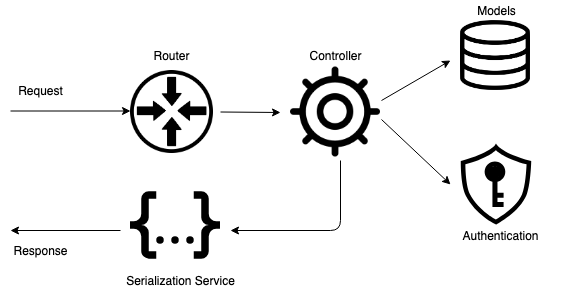
\includegraphics[scale=0.6]{figures/request_test.png}
            \caption{\label{new_arch} Request Lifetime in Backend Service}
          \end{figure}

          Chaque route de l'application est testée, en explorant différent
          scénarios possibles (token d'authentification invalide, action
          non autorisée pour l'utilisateur). On a donc une série de tests
          qui mettent en oeuvre l'intégralité de l'application, avec simplement
          un envoi de requêtes et une comparaison sur les réponses attendues
          de la part de l'application.

      \subsection{Code Coverage - Simple Cov}

        Nous avons choisi d'utiliser Simple Cov en combinaison du testing appliqué
        au Backend. Cet outil permet de mesure le code coverage d'une application
        Ruby et de fournir des informations utiles grâce à une analyse des
        exécutions des tests.\\

        Notre ambition sur la partie utilisateur de Splay ayant été une refonte
        des services en services plus simples et maintenables, il était dès lors
        simple et évident d'atteindre une couverture totale avec une suite de tests,
        et avons décidé d'utiliser cet outil.

      \subsection{Code Quality - Rubocop}

        Dernière partie de l'ensemble d'outils destinés à assurer la qualité du
        service, nous avons utilisé Rubocop, un outil d'analyse statique du code
        (linter) permettant de détecter les enfreintes à une série de codes
        de conduites en termes de style et pratiques (méthodes trop longues,
        trop d'instanciations de variables, trop d'embranchements dans le code,
        ...).

    \section{Testing in Daemons}


    \section{Integration Testing}

      Afin de pouvoir tester automatiquement le projet dans son ensemble, nous
      avons aussi voulu développer des tests fonctionnels. Ces tests seraient
      relativement simples mais suffisamment complets pour s'assurer de
      tester de manière globale les features développées sur le système, et
      il suffisait pour cela de transcrire nos scénarios d'utilisation en
      scénarios de tests.\\

      Pour ceux-ci, nous n'avons pas utilisé de technologie complexe et avons
      estimé qu'une série de scripts en Bash était plus que suffisante pour
      parvenir à nos fins. Bash ne permettrait pas de tester des scénarios
      utilisateurs à travers l'application web, mais étant donné que celle-ci
      utilise exactement la même API fournie par le Backend que l'application
      CLI, nous pouvions donc simuler les actions utilisateurs via celui-ci (
      et c'est en partie pour cette raison que nous avons conservé une
      application CLI dans le projet).\\

      Les tests d'intégration ont été placés dans un dossier spécifique à la
      racine du projet Splay, et achèvent les actions suivantes pour chaque
      test : \\

      \begin{itemize}
        \item Nettoyage des containers
        \item Rebuild des différents services listés dans le docker-compose
        \item Démarrage des services
        \item Execution de commandes via le CLI
        \item Vérification de la réponse retournée par le CLI et affichage du
        succès ou de l'erreur de cette phase de test dans le terminal
      \end{itemize}

      {\color{red} Faire le lien avec les scénarios du début}\\

      Cette manière de procéder et le fait d'utiliser nos scénarios utilisateurs
      pour déterminer les actions décrites dans les tests nous permettent de
      nous assurer et de valider que l'implémentation de nos features est
      fonctionnelle tout au long du projet de la vie de Splay. De plus, ces
      tests viennent ajouter une couche de validation supplémentaire par rapport
      aux tests ciblant les différents services individuellement. On se retrouve
      ici avec des tests qui font intervenir chaque service dans un cas concret
      de fonctionnement du projet, et permet donc aussi de tester les interactions
      entre ceux-ci.


    \section{Continuous Integration}

      Encore dans un soucis de qualité, les differents service ont été placés
      sur la plateforme d'intégration continue Travis CI, le but étant de se
      servir des hooks fournis par Travis sur l'exécution des tests.\\

      Splay étant un projet open source, et que nous espérons voir évoluer, son
      développment collaboratif se fera inévitablement à travers l'organisation
      Github dans laquelle les repositories se trouvent.\\
      Les hooks Travis permettent, dans le cadre d'une pull request, d'obtenir
      une review de l'exécution de tests sur la branche qui demande à être
      mergée, et de s'assurer que le build est sain.

    \section{Overall Testing Suite}

      Here is a figure detailing the whole Splay project with the different
      test suites and procedures that have been described in the previous
      sections so that the reader can get the grasp on the overall
      organisation of this.

      \begin{figure}[H]
        \centering
        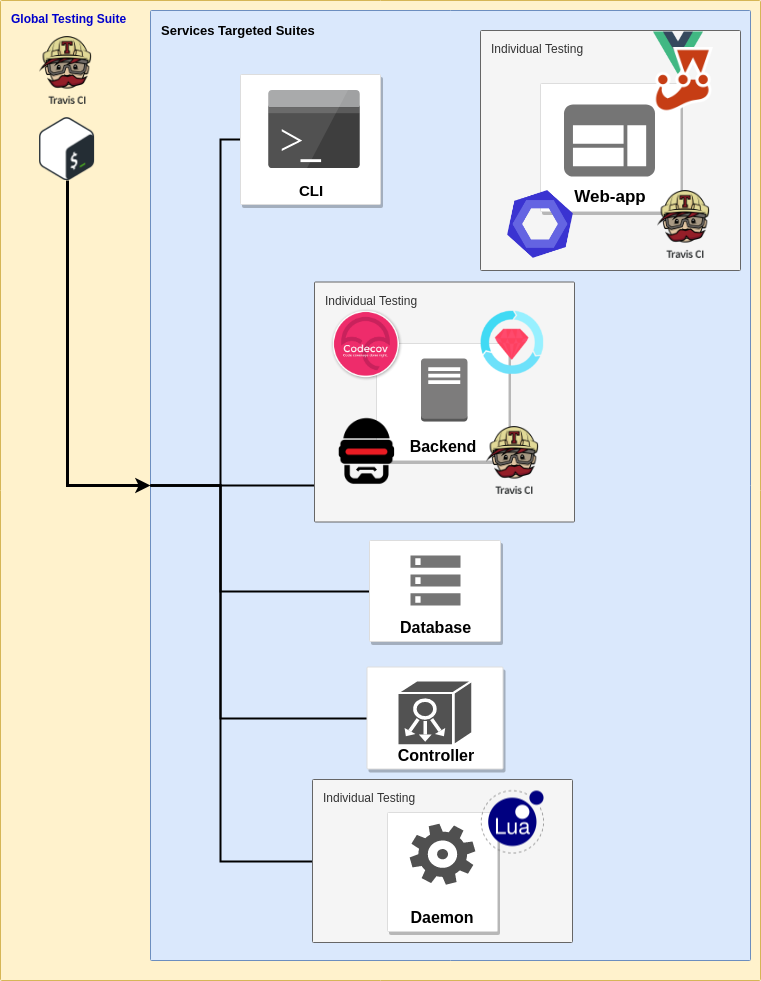
\includegraphics[scale=0.6]{figures/global_testing.png}
        \caption{\label{prev_arch} Global Testing in Splay}
      \end{figure}

  \chapter{Conclusion}

    \section{Objective vs Done}

    \section{}

  \chapter{Improvements}


  \nocite{*}
  \bibliographystyle{plain}
  \bibliography{biblio.bib}




  % Back cover page
  \backcoverpage

\end{document}
